
\section{Анализ работы ЭЦН}

Сегодня доминирующая доля нефти в РФ добывается при помощи ЭЦН. Требуется детальное понимание основных особенностях эксплуатации данного оборудования, режимах работы, возможных осложнениях по причине высокой вязкости продукции, газосодержания, механических примесей и т.д.

Наиболее ценную информацию о работе насоса может дать его характеристика: зависимость параметров работы ЭЦН - напора, потребляемой мощности, перепада давления, КПД, от подачи (дебита скважины)

Для анализа работы скважины, оснащенной УЭЦН, требуются следующие исходные данные

\begin{enumerate}
	\item Физико - химические свойства флюида
	\item Данные по скважине
	\item Данные по ЭЦН
	\item Параметры пласта
\end{enumerate}

PVT свойства задаются аналогично предыдущим упражнениям, а для параметров, характеризующих скважину, приняты следующие обозначения

$H_{mes}$ - глубина скважины измеренная (вдоль ствола скважины), м

$H_{mes}- H_{vert}$ - удлинение ствола скважины, м

$H_{pump}$ - глубина спуска насоса, м

$ID_{cas}$ - внутренний диаметр обсадной колонны, мм

$OD_{tub}$ - внешний диаметр НКТ, мм

$ID_{tub}$ - внутренний диаметр НКТ, мм

$D_{intake}$ - диаметр приемной сетки ЭЦН, мм

$P_{buf}$ - буферное давление, атм

$P_{intake}$ - давление на приеме ЭЦН, атм

$T_{intake}$ - температура на приеме ЭЦН, С

$P_{dis}$ - давление на выкиде ЭЦН, атм

$P_{wf}$ - давление на забое, атм

$Q_{liq}$ - дебит жидкости в поверхностных условиях, м3/сут

$f_w$ - обводненность в поверхностных условиях, \%

\begin{figure}[h!]
	\center{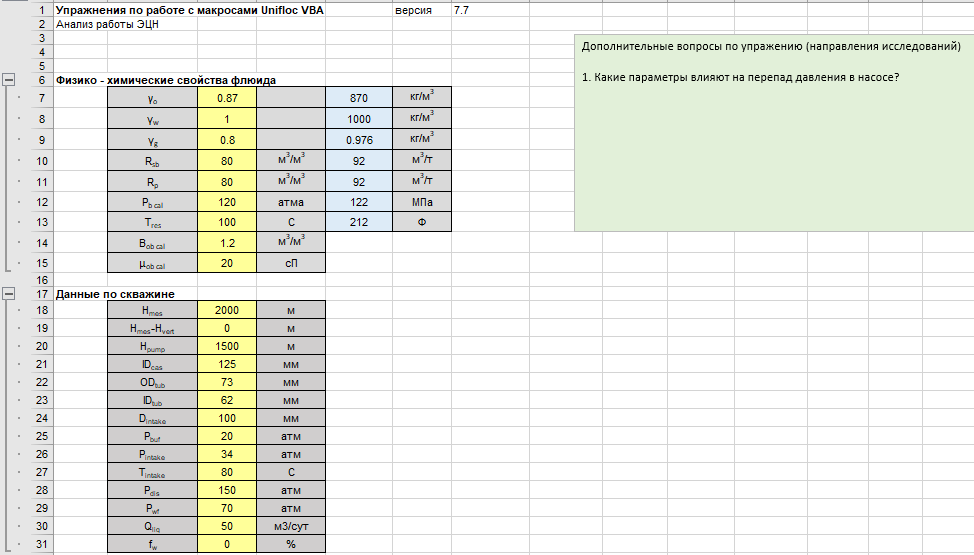
\includegraphics[width=1\linewidth]{Ex70_1}}
	\caption{Исходные данные для свойств флюида и параметров скважины}
	\label{ris:Ex70_1}
\end{figure}

Параметры, описывающие ЭЦН: 

ЭЦН $Q_{nom}$ - номинальная подача ЭЦН, м3/сут

ЭЦН $H_{nom}$ - номинальная напом ЭЦН, м

$F$ - частота питающего тока двигателя, Гц

ЭЦН $ID$ - идентификационный номер насоса (по формуле, см. ниже), находящийся в базе \unf

ЭЦН имя - обозначение насоса: название, габарит и номинальная подача (по формуле, см. ниже)

ЭЦН $Q_{max}$ - максимальная производительность насоса (по формуле, см. ниже), м3/сут

Ступени - количество ступеней, исходя из общего напора ЭЦН и напора одной ступени (по формуле, см. ниже), шт

$K_{sep_ГС}$ - коэффициент сепарации газосепаратора, \%

$P_{sep}$ - давление сепарации, атм

$T_{sep}$ - температура сепарации, С

Данные о пласте:

$P_{res}$ - пластовое давление, атм

$PI$ - коэффициент продуктивности скважины (по формуле, см. выше в упражнении IPR), м3/сут/атм

$\frac{dT}{dL}$ - геотермический градиент, град / 100 м

\begin{figure}[h!]
	\center{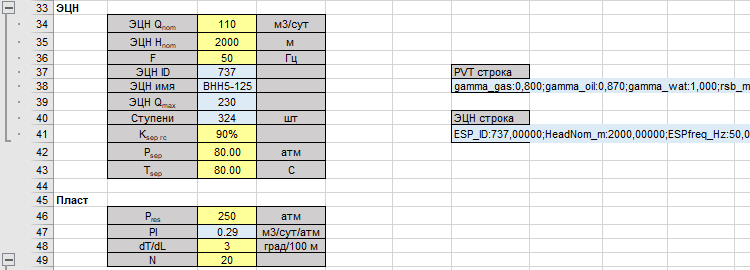
\includegraphics[width=1\linewidth]{Ex70_2}}
	\caption{Исходные данные для ЭЦН и пласта}
	\label{ris:Ex70_2}
\end{figure}

Для получения идентификационного номера насоса в базе \unf \ была использована формула

{ \small  \texttt{=ESP\_id\_by\_rate(Q\_ESP\_)}}

Для определения обозначения ЭЦН

{ \small  \texttt{=ESP\_name(C37)}}

Расчет максимально возможного дебита

{ \small  \texttt{=esp\_max\_rate\_m3day(Freq\_;PumpID\_)*1}}

Количество ступеней

{ \small  \texttt{=ЦЕЛОЕ(Head\_ESP\_/ESP\_head\_m(Q\_ESP\_;1;;PumpID\_))
}}

Также для удобства использования параметры насоса: ID, напор и рабочая частота, зашифровываются в строку с помощью функции

{ \small  \texttt{=ESP\_Encode\_string(PumpID\_;Head\_ESP\_;Freq\_)}}

Свободный газ негативно влияет на работу ЭЦН. В ячейке D51 вычисляется объемная доля газа на приеме газосепаратора с помощью формулы

{ \small  \texttt{=MF\_gas\_fraction\_d(Pintake\_;Tintake\_;fw\_;PVTstr)}}
 
В соседней ячейке D50 для удобного расположения задается вязкость в сПуаз

Построение напорной характеристики данного насоса выполняется с учетом вязкости перекачиваемой продукции. Реализованный метод пересчета характеристики с воды на вязкую жидкость Института Гидравлики позволяет учитывать изменение рабочих параметров из-за данного негативного влияния.

Для вычисления напора в метрах водного столба в ячейке D54 воспользуйтесь формулой

{ \small  \texttt{=ESP\_head\_m(C54;NumStage\_;Freq\_;PumpID\_;mu)}}

КПД ЭЦН в долях единиц 

{ \small  \texttt{=ESP\_eff\_fr(C54;NumStage\_;Freq\_;PumpID\_;mu)}}

Потребляемую ЭЦН мощность в Вт

{ \small  \texttt{=ESP\_Power\_W(C54;NumStage\_;Freq\_;PumpID\_;mu)}}

\begin{figure}[h!]
	\center{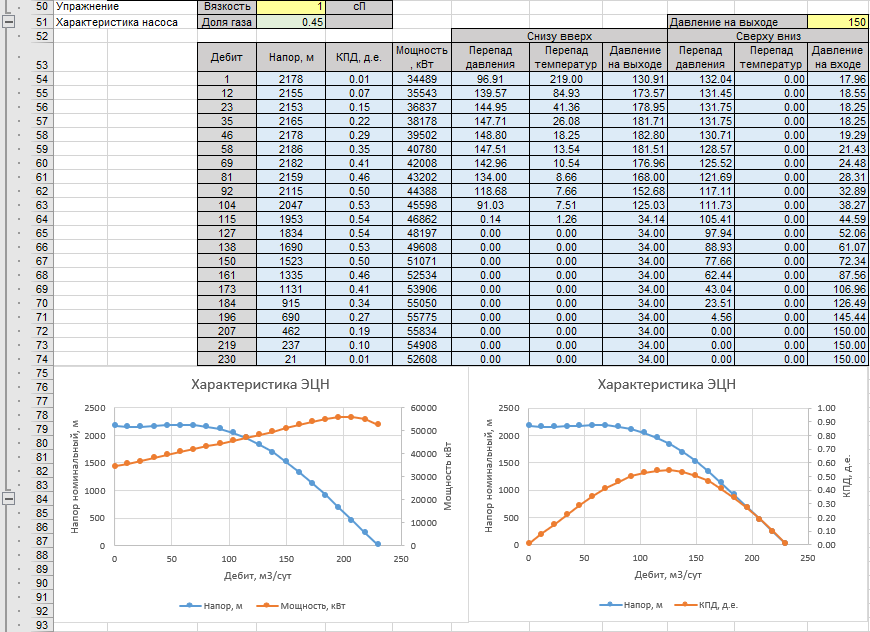
\includegraphics[width=1\linewidth]{Ex70_3}}
	\caption{Напорные характеристики ЭЦН с поправкой на вязкость}
	\label{ris:Ex70_3}
\end{figure}

Расчет перепада давления, развиваемого насосом, может происходить методом "сверху-вниз" \  и "снизу-вверх" \ , при этом расчет перепада температур только методом "снизу-вверх". Функция расчета перепада давления и температуры возвращает массив значений, т.е. одновременно перепад давления и температуры. Кроме того, входным параметром для данной функции является направление расчета. Для вычисления выделите диапазон G54:H54, наберите формулу

{ \small  \texttt{=ESP\_dP\_atm(C54; fw\_; Pintake\_; NumStage\_; Freq\_; PumpID\_; PVTstr; Tintake\_; 0)}}

и после нажмите сочетание клавиш  Ctrl+Shift+Enter. Далее протяните результат до полного заполнения двух столбцов.

Зная давление на приеме и перепад давления в ЭЦН, давление на выходе ЭЦН можно легко посчитать по формуле

{ \small  \texttt{=G54+Pintake\_}}

Предварительно задав давление на выходе ЭЦН в ячейке L51 возможно посчитать перепад давления методом "сверху-вниз"\ аналогичным образом по формуле

{ \small  \texttt{=ESP\_dP\_atm(C54; fw\_; Pdis\_; NumStage\_; Freq\_; PumpID\_; PVTstr; Tintake\_; Tintake\_; 0)}}

И давление на входе, зная давление на выходе и перепад давления

{ \small  \texttt{=Pdis-J54}}

\begin{figure}[h!]
	\center{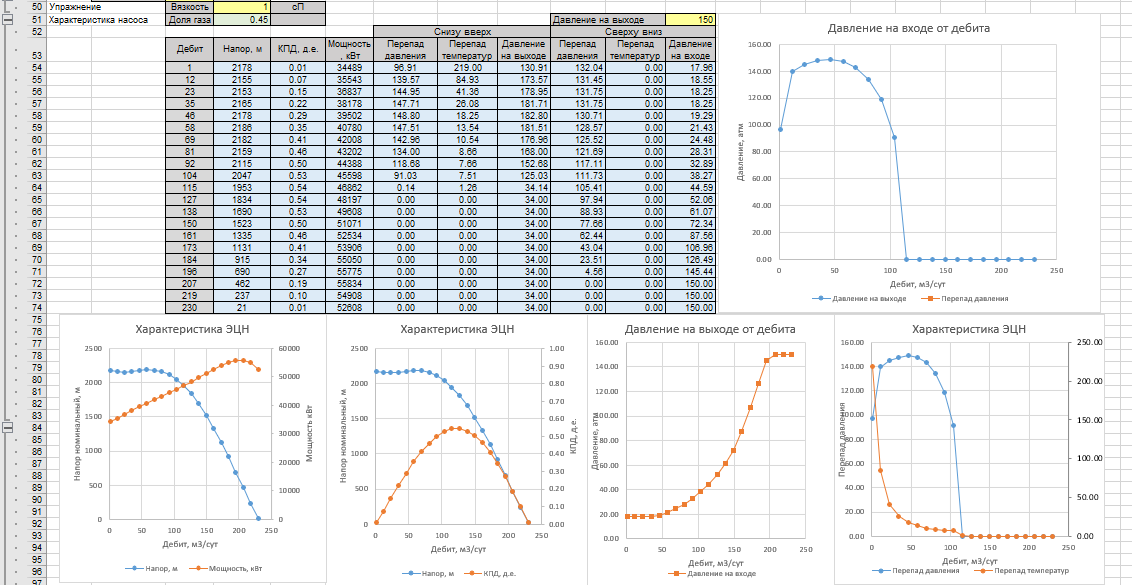
\includegraphics[width=1\linewidth]{Ex70_4}}
	\caption{Расчет перепада давления и температур в ЭЦН в зависимости от дебита}
	\label{ris:Ex70_4}
\end{figure}

Вопросы для упражнения:

\begin{enumerate}
	\item Какие параметры влияют на перепад давления в насосе?
	\item Насколько сильно влияет вязкость на напорные характерситики ЭЦН?
	\item Как влияет на работу ЭЦН изменение частоты?
\end{enumerate}


\section{Анализ работы ПЭД}

Упражнение показывает характеристики погружного асинхронного электрического двигателя, применяемого в УЭЦН.

Также стоит отметить, что расчетные функции предназначаются для образовательных целей. Детального сопоставления расчетных характеристик с фактическими не проводилось. (06.2019)

Для выполнения упражнения необходимо задать параметры электродвигателя

$U_{nom}$ - номинальное напряжение ПЭД, В

$F_{nom}$ - номинальная частота тока, Гц

$I_{nom}$ - номинальная сила тока, А

$ID$ - способ инициализации данных двигателя. 1 - по фактическим значениям параметров (по паспорту), 2 - по схеме замещения Гридина

А также рабочее напряжение $U$, В и рабочую частоту тока $F$, Гц

После этого в ячейке С10 будет произведен расчет номинальной мощности ПЭД с помощью функции

{ \small  \texttt{=Motor\_Pnom\_kW(Unom;Inom;Fnom;ID)}}

\begin{figure}[h!]
	\center{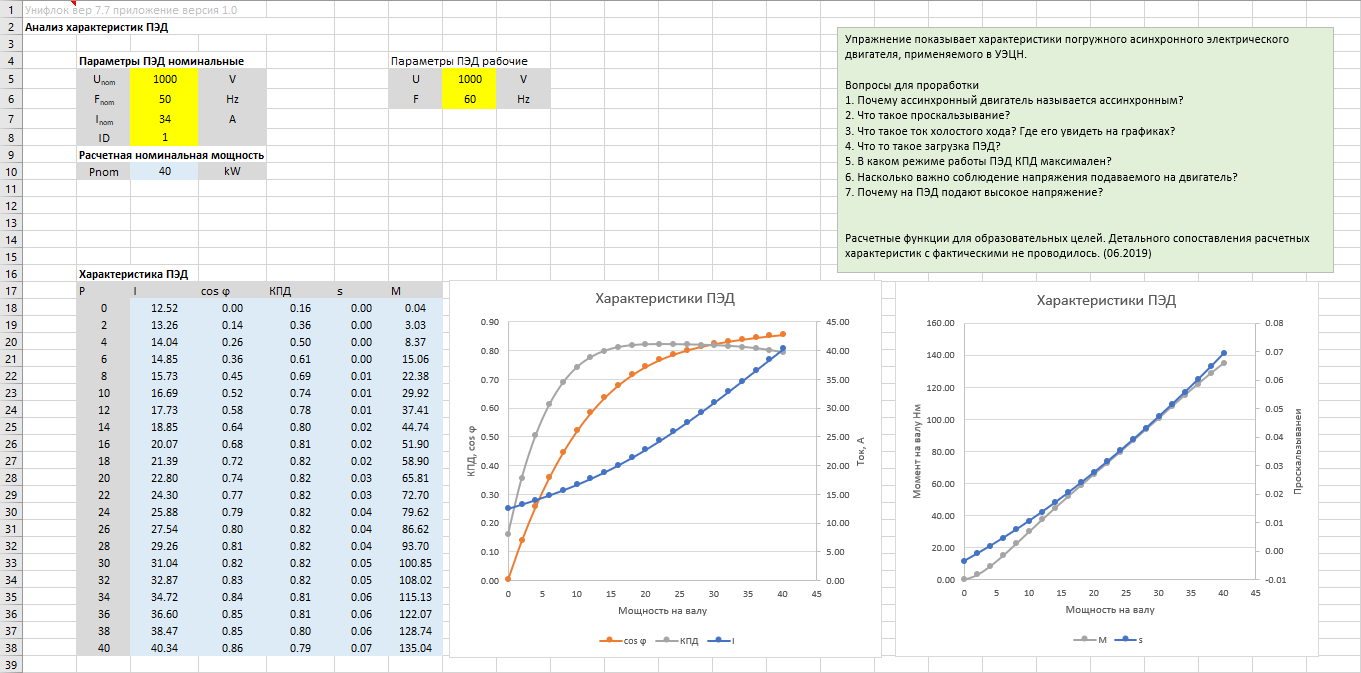
\includegraphics[width=1\linewidth]{Ex80_1}}
	\caption{Исходные данные ПЭД и различные характеристики в зависимости от мощности на валу}
	\label{ris:Ex80_1}
\end{figure}

Для построения характеристики ПЭД (параметры двигателя от мощности на валу $M$) воспользуйтесь следующими формулами

Определение тока двигателя $I$, A

{ \small  \texttt{=motor\_I\_A(B18;F;U;Unom;Inom;Fnom;ID)}}

Расчет $cos \varphi $

{ \small  \texttt{=motor\_CosPhi\_d(B18;F;U;Unom;Inom;Fnom;ID)}}

КПД, д.ед.

{ \small  \texttt{=motor\_Eff\_d(B18;F;U;Unom;Inom;Fnom;ID)}}

Проскальзывание $S$

{ \small  \texttt{=motor\_S\_d(B18;F;U;Unom;Inom;Fnom;ID)}}

Момент на валу $M$, Н*м

{ \small  \texttt{=motor\_M\_Nm(B18;F;U;Unom;Inom;Fnom;ID)}}

\begin{figure}[h!]
	\center{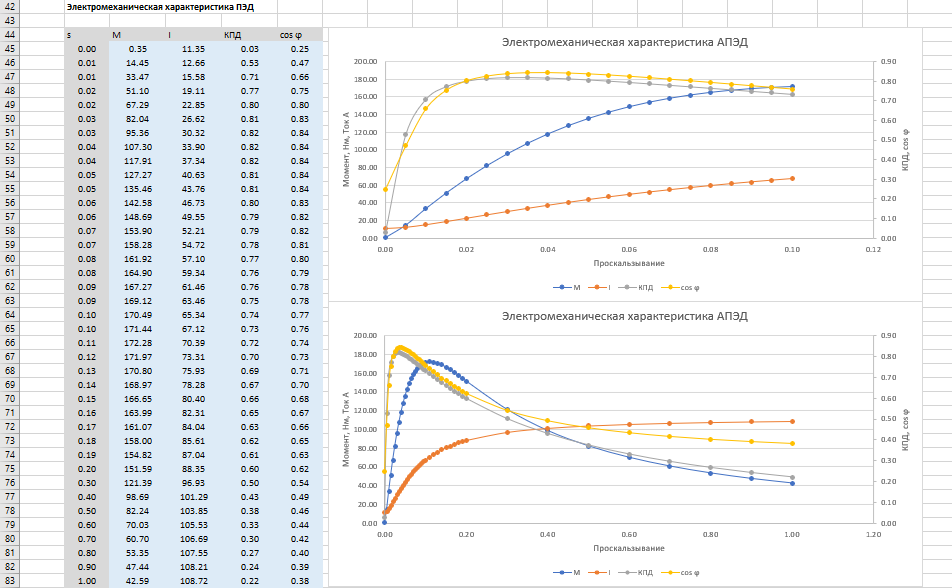
\includegraphics[width=1\linewidth]{Ex80_2}}
	\caption{Электромеханическая характеристика АПЭД}
	\label{ris:Ex80_2}
\end{figure}

Для расчета электромеханической характеристики АПЭД (параметры двигателя в зависимости от проскальзывания $S$) используйте формулы

Момент на валу $M$, Н*м 

{ \small  \texttt{=motor\_M\_slip\_Nm(B45;F;U;Unom;Inom;Fnom;0)}}

Сила тока $I$, А

{ \small  \texttt{=motor\_I\_slip\_A(B45;F;U;Unom;Inom;Fnom;0)}}

КПД, д.ед.

{ \small  \texttt{=motor\_Eff\_slip(B45;F;U;Unom;Inom;Fnom;0)}}

Расчет $cos \varphi $

{ \small  \texttt{=motor\_CosPhi\_slip(B45;F;U;Unom;Inom;Fnom;0)}}


\begin{figure}[h!]
	\center{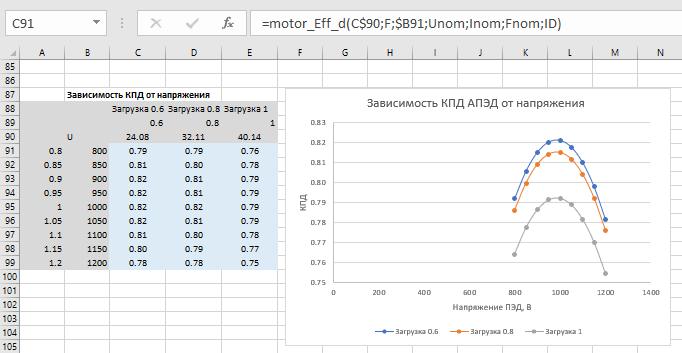
\includegraphics[width=1\linewidth]{Ex80_3}}
	\caption{Зависимость КПД АПЭД от напряжения и загрузки}
	\label{ris:Ex80_3}
\end{figure}

Для проведения исследований по напряжению ПЭД воспользуйтесь следующими формулами для значений загрузки двигателя 0.6, 0.8, 1 

{ \small  \texttt{=motor\_Eff\_d(C\$90;F;\$B91;Unom;Inom;Fnom;ID)}}

{ \small  \texttt{=motor\_Eff\_d(D\$90;F;\$B91;Unom;Inom;Fnom;ID)}}

{ \small  \texttt{=motor\_Eff\_d(E\$90;F;\$B91;Unom;Inom;Fnom;ID)}}

в ячейках C91, E91, D91 соответственно. "Протянув"\ значения Вы можете заполнить таблицу.

Вопросы для упражнения:

\begin{enumerate}
	\item Почему ассинхронный двигатель называется ассинхронным?
	\item Что такое проскальзывание?
	\item Что такое ток холостого хода? Где его увидеть на графиках?
	\item Что то такое загрузка ПЭД?
	\item В каком режиме работы ПЭД КПД максимален?
	\item Насколько важно соблюдение напряжения подаваемого на двигатель?
	\item Почему на ПЭД подают высокое напряжение?
\end{enumerate}